%% For normal draft builds (figs not displayed hence fast compile)
%\documentclass[hyperpdf,nobind,draft,oneside]{hepthesis}
%\documentclass[hyperpdf,nobind,draft,twoside]{hepthesis}

%% For short draft builds (breaks citations by necessity)
%\documentclass[hyperpdf,nobind,draft,hidefrontback]{hepthesis}

%% For Cambridge soft-bound version
\documentclass[hyperpdf,bindnopdf]{hepthesis}
%% For Cambridge hard-bound version (must be one-sided)
%\documentclass[hyperpdf,oneside]{hepthesis}

%% Load special font packages here if you wish
\usepackage{lmodern}
\usepackage{mathpazo}

\usepackage{braket}
\usepackage{SIunits}
\usepackage{acronym}
\usepackage{xspace}
\usepackage{morefloats,subfig,afterpage}
\usepackage{mathrsfs} % script font
\usepackage{verbatim}
\graphicspath{{Figures/Chapter1/}{Figures/Chapter2/}{Figures/Chapter3/}{Figures/Chapter4}{Figures/}}

\newcommand{\Muquans}[0]{\(\mu\)Quans\xspace}
%% Disables warning about Command terminated with a space
% chktex-file 1

\title{Inertial Navigation using Atom Interferometry}
\author{Jimmy Stammers}

%% Doc-specific PDF metadata
\makeatletter%
\@ifpackageloaded{hyperref}{%
\hypersetup{%
pdftitle = {Inertial Navigation using Atom Interferometry},
pdfsubject = {Jimmy Stammers’ PhD thesis},
pdfkeywords = {atom interferometry, navigation, physics, Rubidium},
pdfauthor = {\textcopyright\ Jimmy Stammers},
colorlinks=false,
linkcolor=black
}}{}
\makeatother

\begin{document}

\begin{frontmatter}
    \titlepage[Department of Physics\\
Centre for Cold Matter]{A thesis submitted to Imperial
  College London for partial
fulfillment of the requirements for the degree of Doctor of Philosophy }
\begin{abstract}
    Matter-wave interferometry has enabled high precision measurements of
    inertial forces such as gravity and the
    Coriolis force. This is facilitated by the long-term stability of
    the physical properties of atoms and lasers. Recent experiments have
    demonstrated the operation of portable, robust sensors using atom
    interferometry. This has potential uses in the context of inertial
    navigation, where conventional devices suffer from long-term
    drifts due to bias instability. Furthermore, determining position
    via dead reckoning requires minimisation of dead time between
    measurements. This thesis presents the development of an atom
    interferometer for measuring horizontal accelerations. In this
    configuration, gravity induces motion across
    the laser wavefront, which constrains the tolerable level of
    wavefront distortions. Effective control of the experiment allows
    the interferometer to be operated at a rate of \sivalue{4}{\Hz}. A cold ensemble of $10^6$ atoms in the same
    internal state is prepared in \sivalue{150}{\ms}. The
    interferometer operates
    using a sequence of three laser pulses separated by
    $T=$ \sivalue{25}{\ms} to achieve sensitivity
    to horizontal accelerations. Combining this with a classical
    accelerometer provides a method of correcting for
    vibration-induced noise, as well as determining the interferometer
    fringe order. After an integration time of \sivalue{70}{\s}, the
    sensitivity to horizontal accelerations is better than
    \sivalue{1e-6}{\m\s\tothe{-2}}. Effects which limit this
    sensitivity are discussed.
 \end{abstract}
\begin{declaration}
  I declare that this thesis is the result of my own work. All sources
  used for this work have been clearly referenced in accordance with
  the departmental requirements.   
        \vspace*{1cm}
        \begin{flushright}
        Jimmy Stammers
        \end{flushright}
        \vfill
  The copyright of this thesis rests with the author and is made
available under a Creative Commons Attribution Non-Commercial No
Derivatives licence. Researchers are free to copy, distribute or
transmit the thesis on the condition that they attribute it, that they do
not use it for commercial purposes and that they do not alter,
transform or build upon it. For any reuse or redistribution,
researchers must make clear to others the licence terms of this
work.
\end{declaration}
\begin{acknowledgements}
\noindent
There are many people whose support I wish to acknowledge. Firstly, I would like to thank Ed Hinds for his
supervision and guidance throughout the project. His attention to
detail and desire to understand the experiment from first principles
have taught me a lot about how to approach scientific research. I also
owe a great deal of thanks to the various post-docs I have worked
with. Yu-Hung Lien and Giovanni Barontini were both immensely helpful when I was a new student
and unfamiliar with the techniques required to trap and cool Rubidium
was invaluable. After they moved on, we were soon joined by Indranil
Dutta. As someone who had just come from a well-established
atom interferometry experiment, he was a welcome addition
to our project. I owe him a great deal for everything he taught me
about how to build an interferometer and to diagnose the inevitable
problems along the way. Later on, we were joined by Joe Cotter and
Teodor Krastev, who were both very helpful in developing the
interferometer into a more robust device. Joe was. Theo's expert
Then there are the other students on the Navigator project. It was a
great pleasure working with Xiaxi Cheng as he was always willing to
work on understanding the problem at hand. The next stage of the
project is being undertaken by Shane de Souza and Nicola Bilton. I
have enjoyed working with the both of them and being able to pass on
some of the knowledge that I have learned to them. I wish them all the
best for the continuation of their PhDs. 
\par\noindent 
I have thoroughly enjoyed working as part of CCM. The friendly,
collaborative environment, as well as the social cohesion of the group
is something often hard to come by. I would like to particularly
acknowledge Kyle Jarvis and Dylan Sabulsky. The three of us started
our PhDs together, and I feel that we have a lot of shared experiences
of life as PhD students, both positive and negative. I also owe a
great deal of thanks to Sanja Maricic and Jon Dyne. Without Sanja's
ability to deal with the complex and intricate details of Imperial
College's administration and Jon's expertise at turning
any Inventor design into a precision-engineered component, I am
certain my PhD would have gone much differently.
\par\noindent
Finally, I would like to acknowledge people within my personal life
who have helped me get to where I am today. My parents, Si\^{a}n and
Carl have been very supportive of my choices in life. I am grateful
for everything they have given me. Last, but by no means least, I would
like to thank Vickie for our time together. She has encouraged me to pursue the things I
enjoy and to focus on the positive aspects of work, as well as life. Even when we were thousands of miles apart, she continued to
offer her kind words of encouragement and I will forever be grateful
for her unique support.
\end{acknowledgements}
%\begin{preface}
%    This thesis describes my research on various aspects of\ldots
%\end{preface}

%\begin{frontmatter}
    %   \dedication{For the World}
    %   ...
%\end{frontmatter}

\tableofcontents
\listoffigures
\listoftables
\frontquote{I may not have gone where I intended to go, but I think I
have ended up where I needed to be}{Douglas Adams}

\end{frontmatter}

\begin{mainmatter}
    \chapter{Introduction}\label{chap:intro}
\section{Technology and Quantum Mechanics}
Throughout history, scientific progress has paved
the way towards great technological and societal advances. A
(relatively) modern
example of this is the development of quantum mechanics,
around the start of the 20\textsuperscript{th} century. This led to
vast improvements in the understanding of the physical world at the
microscopic scale. Eventually, the application of quantum theories of
matter and light led
to technological discoveries which have hugely impacted upon
subsequent scientific research, as well as our general lifestyle. These benefits are not always immediately obvious. For
instance, around the time that the laser was
discovered~\cite{Schawlow1958}, it
was believed that a coherent source of light was of little practical
use
outside of spectroscopy. Of course, the widespread use of commercial laser systems in
medicine and telecommunications show that this is not the case.
Another such example is the development of semiconductor electronics, which started with the transistor and has revolutionised
modern life with the plethora of devices seen today. 
\par\noindent
Broadly speaking, these technologies rely on quantum phenomena that
exist within
bulk matter, i.e. macroscopic ensembles of quantum objects. 
These do not exhibit the microscopic quantum phenomena such as
entanglement and interference. They are open systems, which interact strongly with their
environment causing a loss of coherence across the ensemble. For
this reason, there has been a
growth in research that has focused on the control of
individual quantum systems, such as atoms, molecules and photons.
Experimentally, these can be well-isolated from their environment so
that the coherence between quantum states affects the dynamics of the
system. Technologies aimed at controlling quantum systems have
progressed to the point where it is now possible to engineer robust
devices that make use of quantum effects. This is well-known in the
context of quantum computing and quantum cryptography, which offer
many benefits over their classical counterparts. 
\par\noindent
The field of metrology has also shown great increases in measurement
precision using quantum systems. The archetypal example of this is the
atomic clock~\cite{ESSEN1955}, which uses the interference between two internal states
of an atom such as Caesium-13 to
measure their transition frequency. Owing to their frequency
stability, atomic clocks are now used to implicitly define the
second in terms of physical constants and provide a continuous,
precise time scale~\cite{Levine}.

\section{Inertial Navigation}
The ability to measure inertial forces, i.e. accelerations and
rotations, is of
great practical interest. This is strongly motivated by the need for
inertial navigation systems. In general, these make use on on-board
sensors to determine its position using the process of dead reckoning.
The acceleration and rotation are periodically measured and the
position of the object relative to its initial position is determined by
integrating these forces. The accuracy of this method depends upon the intrinsic noise and bias of these devices. These
lead to a position error which grows in time. For instance, the
effects of white noise are discussed in~\cite{Wen2016}. In the context
of this project, the effects of a sensor's stability over time is
discussed more quantitatively using the Allan variance
in~\SectionRef{subsec:allan_variance}.
\par\noindent
Generally, the
position error due to sensor noise can be reduced through statistical
techniques such as Kalman filtering. This produces an un-biased estimate
of the updated position by taking the noise of each sensor into
account. The position error due to a bias must be addressed
separately. A constant acceleration bias, $\epsilon$ leads to a
position error that grows quadratically in time. An initial
calibration of the sensor can remove this bias, but cannot account for
drifts over time. This phenemenon, often termed bias instability, is
the result of effects such as temperature variations and mechanical
strains. This leads to a characteristic time beyond which the
measurement uncertainty is not reduced by averaging the signal. This
problem can be alleviated by regularly correcting for the position
error using an external positioning system, such as \ac{gnss}, and
re-calibrating the sensors.
\subsection{Improving Long-Term Stability with Atom Interferometry}
Experiments over the past few decades have highlighted the prospect of
using cold atoms for precise inertial sensing. Once cooled to the
\sivalue{}{\mu\K} regime, the thermal velocity of an atomic ensemble
is small enough that they can be controlled for durations up to the order
of seconds. Early experiments by Kasevich and Chu into matter-wave
interferometry of Sodium atoms demonstrated the 
It has been suggested that the problem of bias instability can be
overcome by using cold atoms to measure inertial forces.  
For instance, there exist commerically available \ac{mems} devices
which have a noise level of $\sim \sivalue{5}{\mu\g}$ in the
0-\sivalue{100}{\Hertz} bandwidth. Since the noise between successive
measurements is uncorrelated, the position error  After many successive measurem  
\section{Thesis Overview}
This thesis is structured as follows. A theoretical introduction to
matter-wave interferometry and the relevant atomic structure of
\ac{rb87} is presented in~\ChapterRef{chap:theory}. This is followed
by a description of the software that was developed to control the experiment and
acquire data in~\ChapterRef{chap:compinterface}. The subsequent chapters
focus on various experimental aspects of the project. The preliminary
cooling and trapping of \ac{rb87} is presented
in~\ChapterRef{chap:mot}. The techniques used to cool the atoms
further and prepare an ensemble in the same internal state are
explained in~\ChapterRef{chap:atom_prep}. This is followed by the
design and characterisation of an in-vacuum optical system for driving
Raman transitions in~\ChapterRef{chap:raman_optics}. Finally, a
characterisation of acceleration-sensitive interference is given
in~\ChapterRef{chap:atom_int}.




    \chapter{Theory}\label{chap:theory}
\begin{itemize}
    \item Describe general principles of light-matter interaction
    \item Specific cases for laser cooling (doppler/sub-doppler) and Raman transitions 
    \item Lead into atom interferometry
    \item Perhaps split this into two shorter chapters 
\end{itemize}
\section{Overview}\label{sec:theory_overview}
\section{Light-Matter Interactions}\label{sec:theory_lmi}
\section{Laser Cooling of Rubidium-87}
\section{Raman Transitions in Rubidium-87}\label{sec:theory_raman}
\section{Light Pulse Atom Interferometry}\label{sec:theory_atomint}

    \chapter{Experimental Setup}\label{chap:setup}
This chapter provides a description of the hardware that makes up the experiment. Over the course of the project, the complexity of the experiment necessarily increased. The setup is presented in a bottom-up approach, starting from the most fundamental components, to provide a clear overview of the system. \\

\verysubsection{To-Do}
\begin{itemize}\item Figures describing each of the lasers
    \item Describe 3D and 2D MOT setups  
    \item Imaging systems
    \item Microwave synthesisers
    \item Raman Assembly
    \item MOT light distribution
\end{itemize}
\section{Chapter Overview}\label{sec:setup_overview}
The first two sections describe the two commercial laser systems used in this experiment. The \Muquans laser system which generates the light used for cooling and repump in the 2D and 3D \acp{mots}, referred to as the \acs{mot} light. The design and operation of this laser is given in \SectionRef{sec:setup_muquans}. A secondary laser system, built by MSquared, is used to generate light to drive Raman transitions between two hyperfine ground states in \ac{rb87}\footnote{The \Muquans laser also has a pair of lasers designed for driving Raman transitions, but these are not used in this experiment. \SectionRef{sec:setup_msquared} gives an explanation for this.}, otherwise referred to as Raman light. This is described in \SectionRef{sec:setup_msquared}.This is followed by a description of the vacuum chamber in \SectionRef{sec:setup_chamber} which contains both the 2D \ac{mot} (\SectionRef{subsec:setup_2DMOT}) and the 3D \ac{mot} (\SectionRef{subsec:setup_3DMOT}).  
\section{Vacuum Chamber}\label{sec:setup_chamber}
\subsection{The 2D MOT}\label{subsec:setup_2DMOT}
\subsection{The 3D MOT}\label{subsec:setup_3DMOT}
\subsection{Imaging Systems}\label{subsec:setup_imaging}
\subsubsection{CCD Camera}\label{subsubsec:setup_ccd}
\subsubsection{Photodiode}\label{subsubsec:setup_photodiode}

\section{The \Muquans Laser System}\label{sec:setup_muquans}
\verysubsection{To-Do}
\begin{itemize}
    \item Laser Schematic
    \item Plots of lock signals
    \item DDS Serial communication
    \item Power output, stability
    \item Refs for other experiments using Muquans systems
\end{itemize}
All the \ac{mot} light in this experiment was generated by the \Muquans laser \cite{muquansWebPage}. \Muquans is a French laser company that is a spin-off from the Institut d'Optique and Observatoire de Paris. Consequently, their technology has been developed over a long history of performing experiments into atom interferometry using Rubidium. A schematic of this laser system is shown in \FigureRef{fig:muquans_schematic}. The \Muquans laser is comprised of four 1560nm \acp{ECDLs} which are frequency-doubled to produce light at wavelengths close to 780nm. The telecommunications industry, which relies heavily on light in the 1530-1565nm wavelength band for optical communications, has motivated a rapid development in low-noise, robust lasers which are much more stable outside of laboratory conditions than their 780nm counterparts. The requirement for long-term stability of a laser system is one which many applications of quantum mechanics to technology will greatly benefit from by removing a need for frequent maintainence.

\begin{figure}
    \includegraphics{muquans_schematic}
    \caption[\Muquans Laser System Diagram]{Schematic of the \Muquans laser system. Each output laser is derived from a 1560nm \acs{ecdl} (shown in green) which is amplified using an \acs{edfa} and then frequency-doubled to 780nm using a \acs{ppln} crystal. A master laser is locked to the 3,4 crossover in \ac{rb85} and the output lasers are offset-locked to their corresponding frequencies. The dashed region indicates the components used for generating light for the \acp{mots}, which was the only function of this laser for this experiment.}\label{fig:muquans_schematic}
\end{figure}
\subsection{Absolute Frequency Reference}
The purpose of the master laser is to provide an absolute frequency reference so that the MOT light and Raman light can be controlled by comparing the frequency difference of the slave lasers to this. The master laser is locked to the 3,4 crossover in \ac{rb85}, so that the 
\subsection{Generating MOT light}
\subsection{Raman light}
\subsection{Real-time Frequency Control}
\section{The M-Squared Laser System}\label{sec:setup_msquared}
\verysubsection{To-Do}
\begin{itemize}
    \item Schematic
    \item Raman PLL phase-noise
    \item Laser Control
    \item DCS module
\end{itemize}
\subsection{Raman Light}
\section{Raman Optical System}\label{sec:setup_ramanoptics}
\subsection{Vacuum design}\label{subsec:setup_ramandesign}
\subsection{Raman Beam Collimator}\label{subsec:setup_ramancollimator}
\subsection{Retro-reflection Assembly}\label{subsec:setup_ramanmirror}
\section{MOT Light Distribution}\label{sec:setup_lightdist}
\subsection{Optical Fibre Network}\label{subsec:setup_fibrenet}
\subsection{Power Control}\label{subsec:setup_lightpower}

\section{Microwave Field Generation}\label{sec:setup_microwave}
\subsection{Setup}\label{subsec:setup_microwave_setup}
\subsection{Wind-Freak Microwave Synthesiser}\label{subsec:setup_windfreak}arg
    \chapter{Computer Interface}\label{chap:compinterface}
\section{Overview}\label{sec:compinterface_overview}
\begin{itemize}
    \item New MOTMaster software to control experiment
    \item Control system diagram
    \item Interfacing with muquans/msquared lasers
    \item Acquiring data from experiment --- axelsuite
\end{itemize}

\section{MOTMaster}\label{sec:compinterface_motmaster}
\subsection{Hardware Abstraction}\label{subsec:compinterface_hwabstraction}
\subsection{Voltage Pattern Generation}\label{subsec:compinterface_patterngen}
\subsection{Timed Serial Communication}\label{subsec:compinterface_serial}
\subsection{Analogue Voltage Acquisition}\label{subsec:compinterface_mmacquisition}
\subsection{Interfacing with External Software}\label{subsec:compinterface_extsofware}

\section{External Laser Control}\label{sec:compinterface_lasercontrol}
\subsection{Muquans Interface}\label{subsec:compinterface_muquans}
\subsection{M-Squared Interface}\label{subsec:compinterface_msquared}
\subsubsection{Browser-based Control}
\subsubsection{Remote JSON Protocol}

\section{Processing Experimental Data}\label{sec:compinterface_dataprocessing}
\begin{itemize}
   \item Describe real-time processing and visualisation of data 
\end{itemize}
\subsection{Image Processing}\label{subsec:compinterface_imageprocess}
\subsection{Photodiode Voltages}\label{subsec:compinterface_photodidode}
\subsection{MEMS Accelerometer}\label{subsec:compinterface_mems}
    \chapter{Preparing Atoms for Interferometry}\label{chap:atom_prep}
\section{Chapter Overview}
This chapter presents the stages of the experiment which prepare an
ensemble of atoms for interferometry, after they are loaded into the
3D \ac{mot}. After being released from the trap, the atoms are cooled
and launched using a moving molasses, as described
in~\SectionRef{sec:optical_molasses}. Following this, a sequence of
optical and microwaves pulses are used to increase the population in
the \(\ket{1,0}\) ground state and end with an ensemble which has a
narrow velocity spread along the Raman axis. A characterisation of
this is given in~\SectionRef{sec:state_prep}.
\par\noindent
Some sections of this chapter refer to parts of the experiment which
have yet to be introduced. Details on the Raman laser and the
velocity-selective Raman pulse can be found
in~\SectionRef{sec:msquared_laser}
and~\SectionRef{subsec:vel_select}, respectively. A
description of the detection scheme, used to measure the population of
atoms in \(\ket{F=1}\) and \(\ket{F=2}\) is presented
in~\SectionRef{sec:atom_detection}.

\section{Cooling in Optical Molasses}\label{sec:optical_molasses}
{\textbf{Introduce motivation here}}
A low thermal velocity means that the atoms can be interrogated for a
longer time and in the case of atom interferometry, leads to a more
sensitive measurement of acceleration. In addition, the thermal
expansion of the ensemble leads to greater systematic phase shifts due
to effects such as magnetic field gradients and laser wavefront
distortions. The temperature of atoms inside the \ac{mot} is greater
than desired, so further cooling is required before a strong
interferometer signal can be achieved. Temperatures well below that of
the Doppler limit (\sivalue{146}{\micro\kelvin} for \ac{rb87}) can be
reached using the dissipative force that acts on an atom travelling
through a spatially varying electric field. 

\par\noindent
This section describes the work towards to cooling and launching the
atoms in a moving optical molasses. It starts with a motivation for
launching the atoms in~\SectionRef{subsec:launching}. The following
section discusses the control of the intensity and frequency of the
light during the molasses stage of the experiment. A description of
the techniques needed to cool the atoms in a moving molasses is then
given in~\SectionRef{subsec:moving_molasses}. Finally, this section
concludes in~\SectionRef{subsec:molasses_imaging} with measurements of
both the temperature and trajectory of the atom cloud which were
measured using a ballistic expansion method.


\subsection{Motivation for Launching}\label{subsec:launching}
As previously discussed in~\SectionRef{sec:theory_double_int}, there are two pairs of counter-propagating beams which can drive Raman transitions between the two hyperfine ground states. If an atom can be stimulated by both pairs, then the additional trajectories this introduces do not interfere, resulting in a reduction in the fringe visibility. This problem can be avoided by using the fact that the Raman transition is Doppler-sensitive to ensure that the atoms are only driven by one pair of beams. Each pair has an opposite Doppler shift \(\pm \omega_D = \pm \keff.\textbf{v}\) and so their transition frequencies are separated by \(2\omega_D\). Therefore, the atoms are launched so that their centre-of-mass velocity along the Raman axis is large enough to lift the degeneracy of the two Raman transitions. 

%The light used to drive Raman transitions during the exeperiment is launched into the chamber on two orthogonal axes of a \ac{pm} fibre. These are retro-reflected to produce two counter-propagating beams that are orthogonally polarised to the incoming ones. In the absence of \(\pi\)-polarised light, only \((\sigma^+-\sigma^+)\) or \((\sigma^--\sigma^-)\) pairs of polarised beams can drive Raman transitions. If the incoming beams are circularly polarised, then this can occur using counter-propagating pairs of beams which impart momentum \(\pm \hbar \keff\) to an atom. If an atom can be driven by either pair at each interferometer pulse, this results in two interferometer paths, as well as additional trajectories which do not interfere and hence cause a reduction in fringe visibility.
\subsection{Frequency and Power Control}\label{subsec:molasses_control}
A timing diagram illustrating the power and frequency during this
stage of the experiment is shown in \FigureRef{fig:molasses_timing}.
After the atoms are loaded into the \ac{mot}, they are released by
switching off the quadrupole field. Once this field has decayed away,
the frequency and intensity of the cooling light are ramped
adiabatically. The frequency of the cooling light is ramped to
-25\(\Gamma\) over \sivalue{1.4}{\milli\second}. Since the repump
light is generated using an \ac{eom}, the modulation frequency is
simultaneously ramped up to keep this light resonant with the
\trans{1}{2} transition. Additionally, the relative detuning of
counter-propagating \ac{mot} beams is varied so that the atoms are
cooled into a moving molasses
(see~\SectionRef{subsec:moving_molasses}). After this, the intensity
of the light is reduced over \sivalue{5}{\milli\second}. The response
of the output \ac{aom} on the \Muquans laser was calibrated so that we
could apply a voltage ramp that gives an approximately linear
intensity ramp.
\begin{figure}[!htbp]
    \centering
    \fontsize{14pt}{14pt}
    \resizebox{0.7\textwidth}{!}{\input{molasses_timing.pdf_tex}}
    \caption[Molasses stage timing diagram]{Timing diagram for the
    molasses stage of the experiment. After a time \(\tau_\text{a} =
  \sivalue{100}{\milli\second}\), the atoms are released from the
\ac{mot}. The molasses sequence begins \sivalue{3}{\milli\second}
later, once the magnetic field from the \ac{mot} coils has decayed
away. First, the frequency of the cooling light is ramped to \(-25
\Gamma\) over \sivalue{1.4}{\milli\second}. The relative frequencies
of counter-propagating \ac{mot} beams are detuned so that the atoms
are cooled in a moving frame, launching them along a parabolic path
(see~\SectionRef{subsec:moving_molasses}). Next, the intensity of the
\ac{mot} light is reduced linearly over \sivalue{5}{\milli\second}. To
measure the temperature, the atoms are left to expand for a duration
of \(\tau_\text{exp}\) \sivalue{}{\milli\second}, after which they are
imaged using the camera.}
    \label{fig:molasses_timing}
\end{figure}
\subsection{Launching in a Moving Molasses}\label{subsec:moving_molasses}

The configuration for launching atoms along the Raman axis is shown in \FigureRef{fig:moving_molasses}. The forward-propagating beams are blue-detuned by \(+\delta_l\) and the backward-propagating ones are red-detuned by \(-\delta_l\), so that atoms with a velocity along the beam axis of \(\vec{v} = \delta_l \lambda\) are+ resonant with both beams. The frequency of each beam is ramped from the initial value by varying the modulation frequency of its \ac{aom}. This ramp occurs slowly to ensure the atoms are adiabatically accelerated to the resonant velocity, minimising excess heating of the atoms. As there is no pair of \ac{mot} beams along the axis of the Raman beams, the \(\vec{x}\) and \(\vec{y}\) \ac{mot} beams, whose axes are nominally at 45\(^{\circ}\) to the Raman axis, are used to launch the atoms. By controlling the power and alignment of each beam, the net velocity on the atoms will be along the Raman axis. If the detuning of both pairs of beams is the same, then the velocity along the Raman axis is given by \(\vec{v_r} = \sqrt{2} \delta_l \lambda\)~\nocite{Ohshima1995}.
\begin{figure}[!htbp]
    \centering
    \def\svgwidth{0.6\textwidth}\input{moving_molasses.pdf_tex}
    %\resizebox{0.6\textwidth}{!}{\input{moving_molasses.pdf_tex}}
    \caption[Beam configuration for a moving molasses]{Beam configuration for a moving molasses. When counter-propagating beams are detuned from each other, the atoms are slowed to a velocity which balances the frequency of each beam. Along the vertical axis, the beams are detuned by \(\delta_v\) so that the cloud is launched upwards with a velocity \(v_z = \delta_v \lambda\). In the horizontal plane, the \(\vec{x}\) and \(\vec{y}\) beams are detuned by \(\delta_h\) so that the resultant velocity is along the Raman axis \(v_r = \sqrt{2}\delta_h\lambda\). }
    \label{fig:moving_molasses}
\end{figure}
\par\noindent
As well as launching the atoms horizontally, the atoms are launched
vertically so that they do not fall as far under gravity. Since the
atoms remain close to the centre of the beam, where the intensity
across the cloud is more uniform, longer pulse separation times can be
used before the intensity gradient causes a significant dephasing.
This launch is carried out using the \ac{mot} beams that lie along the
vertical \(\vec{z}\) axis. 
%Under an appropriate choice of launch
%velocity, the centre-of-mass trajectory transverse to the Raman beam
%wavefront can be chosen to maximise the interferometer fringe
%visibility. This is presented in further detail
%in~\SectionRef{subsec:launch_contrast}. 
\par\noindent
\subsection{Imaging the Atom Cloud over Time}\label{subsec:molasses_imaging}
Once released from the trap, the atom cloud is free to expand.
Provided that there are no external forces on the atoms from electric
or magnetic fields, the expansion of the cloud is determined by its
thermal velocity distribution. In addition to this, the centre-of-mass
moves due to its initial velocity and acceleration due to gravity. For
the purposes of this discussion, it is worthwhile to consider the
motion of atoms within the ensemble separately to the centre-of-mass
motion as these provide a means of measuring the temperature and
launch velocity, respectively. These were measured by imaging the
distribution of atoms after allowing the cloud to expand in the dark
for a range of expansion times. A typical atom cloud trajectory is
shown in~\FigureRef{fig:molasses_launch}, in which the cloud was imaged
up to \sivalue{76}{\milli\second} after being released from the trap.

\begin{figure}[!htbp]
    \centering
    \includegraphics[width=0.8\textwidth]{molasses_launch}
    \caption[Atom cloud position after launching in a moving molasses]{A series of images showing the trajectory of the atom cloud after being cooled in a moving molasses. The first image was taken \sivalue{7}{\milli\second} after initiating the molasses and a subsequent one every \sivalue{5}{\milli\second}. Each image represents a region of interest of dimensions 1150 \(\times\) 1650 pixels that covers the spatial extent of the atom cloud during the launch.}
    \label{fig:molasses_launch}
\end{figure}
\subsubsection{Measuring the Temperature}
In thermal equilibrium, the velocity distribution of the atoms is
described by a Maxwell-Boltzmann distribution
\begin{equation}
    f(v_x,v_y,v_z) = \left(\frac{m}{2\pi k_B }\right)^{3/2}e^{-\frac{m (v`_x^2+v`_y^2+v`_z^2)}{2 k_B T}}
    \label{eq:mb3D}
\end{equation}
where \(v`_i = v_i - \langle v_i \rangle\) is the difference from the
average velocity. Along a single axis, the velocity distribution is
obtained by integrating over the other velocity components. For the
sake of notation, the following discussion uses \(x\) and \(v_x\) as
labels for position and velocity, but these are interchangeable with
the equivalent components along the other axes.
As~\EquationRef{eq:mb3D} is a product of velocity distributions along
each axis, the velocity distribution along one axis is 
\begin{equation}
    f(v_x) = \left(\frac{m}{2\pi k_B }\right)^{1/2}e^{-\frac{m (v_x-\langle v_x \rangle) ^2}{2 k_B T}}
    \label{eq:mb1D}
\end{equation}
Suppose that there are initially \(n_0 (x) \mathrm{d}x\) atoms within
the region \((x, x+\mathrm{d}x)\), where \(n_0(x) = n(x, t=t_0)\) is
the initial atomic density along one axis. During ballistic expansion,
the atoms redistribute themselves according to their velocity. After a
time \(t\) of free expansion, the position of an atom initially at
\(x\) is \(x + v_x t\). 
Assuming that the number density is initially a Gaussian, with a peak
number density \(n_0(x_0)\) at the centre-of-mass, the number density
at later times is given by a convolution with~\EquationRef{eq:mb1D}
\begin{equation}
        n(x,t) = \int n_0(x_0) \left(\frac{m}{2\pi k_B}\right)^{1/2} e^{-\frac{m (v_x-\langle v_x \rangle)^2}{2 k_B T}} e^{-\frac{(x+v_x t - x_0)^2}{2\sigma_0^2}} \mathrm{d}v_x
        \label{eq:density_time}
\end{equation}
where \(\sigma_0\) is the \(1/e^2\) initial width of the cloud. As a
convolution of two Gaussians, \EquationRef{eq:density_time} is also a
Gaussian, with a \(1/e^2\) width given by
\begin{equation}
    \sigma(t)^2 = \sigma_0^2 + \frac{k_B T}{m} t^2
    \label{eq:expansion_width}
\end{equation}
\par\noindent
\FigureRef{fig:molasses_fit_examp} shows a typical density
profile along each axis, obtained by imaging the cloud on a camera, as
previously described in~\SectionRef{sec:imaging}. The width along each
axis is estimated using a non-linear least squares fit
to~\EquationRef{eq:density_time}.
\FigureRef{fig:molasses_temperature} shows the measured cloud width
over a range of expansion times. For the purposes of
measuring the temperature, the total atom number and the initial cloud
size are not important, so no attempt was made to estimate these. The
initial measurement was made \sivalue{7}{\milli\second} after the end
of the molasses to allow for enough time to re-lock the laser to
\(-0.5\Gamma\) below the \trans{2}{3} transition and align the bias
field to the \(\vec{z}\) axis so that the atoms could be optically
pumped into the \(\ket{2,2}\) state. The width of the cloud along each
axis is estimated using a
non-linear least squares fit to~\EquationRef{eq:density_time}. Then, a
least squares linear fit estimates the temperature along
each axis from the gradient, as per~\EquationRef{eq:expansion_width}.
The measured temperature along the horizontal and vertical axes of the
camera was \(T_x = \sivalue{6.38 \pm 0.11}{\micro\kelvin}\) and \(T_y =
\sivalue{6.38 \pm 0.09}{\micro\kelvin}\), respectively.  
\begin{figure}[htpb]
  \centering
  \includegraphics[width=0.8\linewidth]{molasses_fit_examp.pdf}
  \caption[Integrated pixel counts during ballistic expansion.]{Integrated pixel count for a single image during ballistic
  expansion. The dashed lines indicate non-linear least squares fits
to a Gaussian function.}
  \label{fig:molasses_fit_examp}
\end{figure}
\begin{figure}[!htbp]
    \centering
    \includegraphics[width=0.8\textwidth]{temperature_launch}
    \caption[Temperature measurement using ballistic expansion]{Atom
    cloud temperature using a ballistic expansion measurement. After
  molasses, the cloud is left to expand in the dark and in a region of
close to zero magnetic field. A least-squares linear fit of
\(\sigma(t)^2\) is used to estimate the temperature
using~\EquationRef{eq:expansion_width}.  The
gradient from the fits for the horizontal (blue) and vertical (orange)
axes are  \(T_x = \sivalue{6.38 \pm0.11}{\micro\kelvin}\) and \(T_y =
\sivalue{6.38\pm0.09}{\micro\kelvin}\).}
    \label{fig:molasses_temperature}
\end{figure}

\subsubsection{Measuring the Launch Trajectory}
The same method used to measure the temperature of the cloud can also
be used to measure the position of the centre-of-mass. In this case,
the quantity of interest is \(\langle x(t)\rangle\). Since the cloud
is in free-fall, the trajectory for the centre-of-mass is then given
by the well-known equation-of-motion for a particle moving under
constant acceleration
\begin{equation}
    \langle x(t) \rangle = \langle x(0) \rangle + v_x t + \frac{1}{2} a_x t^2
    \label{eq:position_free}
\end{equation}
where \(v_i\) is the initial velocity along the given axis and \(a_i\)
is the acceleration.
\par\noindent
To launch the atoms both vertically and horizontally (along the axis
parallel with the Raman light), the \((z_+, z_-)\) \acp{aom} were
ramped so that the relative frequency difference between each beam was
\(2\times\)\sivalue{320}{\kilo\hertz} and the \(x\) and \(y\) \ac{aom}
frequencies were ramped to give a frequency difference of \(2\times
\sivalue{75}{\kilo\hertz}\) between the horizontal \ac{mot} beams.
\FigureRef{fig:molasses_launch} is a plot of the measured
centre-of-mass position along the horizontal and vertical camera axes
over time. A linear least-squares fit
to~\EquationRef{eq:position_free} gives a vertical launch quantities
of \(v_v = \sivalue{25.0\pm0.24}{\centi\meter\per\second}\) and \(a_v
= \sivalue{-9.40\pm0.051}{\metre\per\second\squared}\) and \(v_h =
\sivalue{7.39\pm0.14}{\centi\meter\per\second}\) and \(a_h =
\sivalue{-0.32\pm0.036}{\metre\per\second\squared}\) along the
horizontal axis. 
\begin{figure}[!htbp]
    \centering
    \includegraphics[width=0.8\textwidth]{molasses_position}
    \caption[Atom cloud centre-of-mass over time]{Measured
    centre-of-mass position over time. The horizontal component of the
  position is shown in blue and the vertical in orange. Each
trajectory is fit to~\EquationRef{eq:position_free} to estimate the
launch velocity. The best-fit values are \(v_v =
\sivalue{25.0\pm0.24}{\centi\meter\per\second}\) and \(a_v =
\sivalue{-9.40\pm0.051}{\metre\per\second\squared}\) along the
vertical axis and \(v_h =
\sivalue{7.39\pm0.14}{\centi\meter\per\second}\) and \(a_h =
\sivalue{-0.31\pm0.036}{\metre\per\second\squared}\) along the
horizontal.}
    \label{fig:molasses_position}
\end{figure}
\par\noindent
When compared to the expected velocities from the detunings,
\(v^{(l)}_v = \sivalue{24.96}{\centi\metre\per\second}\) and
\(v^{(l)}_h = \sivalue{5.85}{\centi\metre\per\second}\), the measured
horizontal velocity is far greater than expected. This can be
explained by a residual magnetic field, that is not cancelled using
the bias coils. In the presence of a magnetic field, atoms cooled in
an optical molasses are decelerated to a velocity at which the Zeeman
shift is cancelled by the Doppler shift. This velocity-selective
resonance depends on the
orientation of the magnetic field to the polarisation of the light. In
a one-dimensional optical molasses, a resonance occurs at
\(v_\text{res}^{(1)} = - \mu_B g_F B/\hbar k\) when the magnetic field
is aligned with the wavevector of the light \cite{VanderStraten1993}.
When the field is aligned at an arbitrary angle an additional
resonance at \(v_\text{res}^{(2)} = - \mu_B g_F B/2\hbar k\) is
present, due to additional \(\left(\sigma^{\pm}-\pi\right)\)
transitions~\cite{Chang2002}. A residual field along the Raman axis of
\sivalue{20}{\milli\gauss} would shift the resonance along \(\vec{x}\)
and \(\vec{y}\) by \sivalue{1.09}{\centi\metre\per\second}
corresponding to a velocity of \sivalue{1.54}{\centi\metre\per\second}
along the Raman axis. The magnetic field inside the chamber is
controlled using bias coils and no attempt was made to cancel magnetic
field gradients. It is plausible that a residual field of this
magnitude is a result of a magnetic field gradient.

\section{State Preparation}\label{sec:state_prep}
After the atoms have been cooled in an optical molasses, the
population will mostly be distributed across the \(\ket{F=2}\) level,
along with a small fraction distributed across the \(\ket{F=1}\)
level. The Raman transition only couples the \(\ket{1,0}\) and
\(\ket{2,0}\) states, so atoms in the other hyperfine ground states
cannot participate in the interferometer. In fact, since the
individual Zeeman sub-levels are not resolved during detection, these
background atoms result in a loss of fringe visibility. One way to
overcome this is to apply a pulse of light resonant with the
\trans{2}{3} transition to push the non-participating atoms out of the
interferometer detection region. Of course, this must be done after
applying a Raman pulse to transfer an ensemble of atoms from
\(\ket{2,0}\) into \(\ket{1,0}\). In this simple scheme a large
fraction of the atoms are removed, which is undesirable since
measurements of a low number of atoms are inherently more uncertain
due to shot number fluctuations. 
\par\noindent
The following section discusses a method of preparing the atoms to
increase the population in the \(\ket{1,0}\) ground state. An overview
of the scheme is given in~\SectionRef{subsec:prep_schemes}. This is
followed by a discussion of the initial steps which optically pump
atoms into the \(\ket{1,0}\) state
in~\SectionRef{subsec:optical_pumping}. A description of the microwave
pulse used to drive atoms into the \(\ket{F=2}\) level is given
in~\SectionRef{subsec:microwaves}. This section concludes with the
method used to blow away the atoms which do not contribute to the
interferometer in~\SectionRef{subsec:blow_away}. A key step which has
been omitted is the velocity-selective Raman pulse. This is described
in more detail later, in~\SectionRef{subsec:vel_select}.
\subsection{Schemes for Preparation}\label{subsec:prep_schemes}
The scheme used to prepare atoms in the \(\ket{1,0}\) state is the
following:
\begin{enumerate}
    \item Light resonant with the \trans{2}{2} transition pumps atoms into the \(\ket{F=1}\) level
    \item Light resonant with the \trans{1}{0} transition drives (\(\sigma^{\pm}\)) transitions to pump atoms into the \(\ket{1,0}\) dark state
    \item A microwave $\pi$-pulse transfers atoms to \(\ket{2,0}\)
    \item A Raman $\pi$-pulse transfers atoms with a narrow velocity spread back to \(\ket{1,0}\)
    \item The atoms which remain in \(\ket{F=2}\) are blown away
\end{enumerate}
A diagram of the population of each hyperfine ground state and the
laser frequencies used to drive these transitions is given
in~\FigureRef{fig:state_prep}. With the exception of step 4, the light
is provided by the \Muquans laser using the \ac{mot} collimators
aligned to the vertical \(\vec{z}\) axis. The frequency of the cooling
laser and the repump sideband are set so that the relevant transitions
for steps 1 and 2 are addressed. As the \(\ket{F=1}\) light is a
sideband of the \(\ket{F=2}\) light, it is not possible to blow away
atoms in \(\ket{F=1}\) without also blowing away atoms in
\(\ket{F=2}\). This problem is overcome by using microwave pulses to
drive atoms up to \(\ket{F=2}\) before velocity selection.
\par\noindent
A timing diagram of the state preparation sequence is shown
in~\FigureRef{fig:state_selection_timing}, which indicates the
duration for which each optical or microwave pulse is applied, as well
as the direction of the applied magnetic field. The field is switched
slowly over \sivalue{2}{\milli\second} (which is omitted from the
diagram) to preserve the spin state of each atom. 
\begin{figure}[!htbp]
    \centering
    %\def\svgwidth{0.8\textwidth}
    \fontsize{24pt}{24pt}
    \resizebox{0.8\textwidth}{!}{\input{state_selection.pdf_tex}}
    \caption[State preparation pulse sequence]{Sequence of optical and microwave pulses used to prepare an ensemble of atoms in \(\ket{1,0}\). The red arrows indicate optical transitions to and from \(\ket{F=2}\) and equivalently for the blue arrows and \(\ket{F=1}\). A residual population in the \(\ket{1,\pm 1}\) states is present, which contributes to a background during the interferometer.}
    \label{fig:state_prep}
\end{figure}
\begin{figure}[!htbp]
    \centering
    %\def\svgwidth{0.5\textwidth}
    \fontsize{14pt}{14pt}
    \resizebox{0.6\textwidth}{!}{\input{state_selection_timing.pdf_tex}}
    \caption[State selection timing schematic]{Timing diagram for state selection sequence. The durations labelled are indicative of the time required to drive the atoms into the desired state at each step. After the \trans{1}{0} pumping, the magnetic field is re-oriented along the Raman axis \(\vec{r}\). The \sivalue{2}{\milli\second} field switching time has been omitted.}
    \label{fig:state_selection_timing}
\end{figure}
\subsection{Optically Pumping the Atoms}\label{subsec:optical_pumping}
\subsubsection{Driving the \trans{2}{2} transition}
After the molasses, the frequency of cooling light is
\sivalue{150}{\mega\hertz} below the \trans{2}{3} transition. This can
off-resonantly excite an atom to the \(\ket{F'=2}\) excited level, but
the small scattering rate means that on average, an atom will need to
scatter many photons before it is pumped into the \(\ket{F=1}\) level.
Therefore, to minimise the heating during this pumping process, the
frequency of the cooling light is resonant with the \trans{2}{2}
transition.
\par\noindent
\FigureRef{fig:step1_pumping} shows the population in the two
hyperfine ground states as the duration of the \trans{2}{2} light is
increased. The rate at which atoms are pumped into \(\ket{F=1}\)
increases with the strength of the applied magnetic field. At zero
field, there exists a dark state which is a coherent superposition of
the \(\ket{2,m_F}\) states~\cite{Berkeland2002}. Applying a magnetic
field lifts the degeneracy between the Zeeman sub-levels so that this
dark state is no longer stationary. The evolution rate of this dark
state, and hence pumping rate, increases with an increasing Zeeman
shift. At a field strength of \sivalue{3}{\gauss}, the atoms can be
pumped into \(\ket{F=1}\) in less than \sivalue{5}{\micro\second}.
\begin{figure}[!htbp]
    \centering
    \includegraphics[width=0.7\textwidth]{step1_pumping}
    \caption[Ground state distribution during \trans{2}{2} pumping]{Population across the two hyperfine ground states after \trans{2}{2} pumping under various magnetic field strengths. The $\smalltriangledown$ ($\circ$) markers indicate the population in $\ket{F=2}$ ($\ket{F=1})$. The red, blue and green series correspond to field strengths of \sivalue{-0.16}{\gauss}, \sivalue{1.67}{\gauss}, and \sivalue{3}{\gauss}, respectively.}
    \label{fig:step1_pumping}
\end{figure}
\subsubsection{Driving the \trans{1}{0} transition}
After this first pumping step, the atoms are distributed across the
Zeeman sub-levels in \(\ket{F=1}\). The next pulse of light is used to
increase the population in \(\ket{1,0}\) by driving \trans{1}{0}
transitions. During this time, the \trans{2}{2} light remains on which
helps to prevent atoms from populating the \(\ket{F=2}\) level through
off-resonant \trans{1}{1} excitations. The magnetic field present
means that the circularly-polarised \(\vec{z}\) \ac{mot} beams only
drive \(\sigma^{\pm}\) transitions, so the \(\ket{1,0}\) state is in
principle a dark state. 
\par\noindent
The distribution of atoms across the Zeeman sublevels was measured
using a microwave pulse to drive atoms into the \(\ket{F=2}\) level,
which is described in~\SectionRef{subsec:microwaves}. For each \(\pi\)
microwave transition, the frequency of the microwave field was varied
to find the resonant frequency. The resulting spectra for \(m_F = -1\)
and \(m_F = 0\) are shown in~\FigureRef{fig:step2_microwave_spec},
both with and without applying light to pump into the \(\ket{1,0}\)
state.  The 0 \(\rightarrow\) 0 clock transition is detuned from the
hyperfine splitting frequency due to the applied magnetic field,
giving a second-order Zeeman shift of
\sivalue{515}{\hertz\per\gauss\squared}. The measured shift of
\sivalue{5.6}{\kilo\hertz} corresponds to a field strength of
\sivalue{3.3}{\gauss}.
\begin{figure}[!htbp]
    \centering
    \def\svgwidth{\columnwidth}
    \subfloat[][]{\scalebox{0.5}{\includegraphics{step2_mf0}}\label{fig:step2_mf0}}\\
    \subfloat[][]{\scalebox{0.5}{\includegraphics{step2_mf1}}\label{fig:step2_mf1}}
    \caption[\(m_F\) populations before and after \trans{1}{0} pumping]{Population of atoms in (a) \(\ket{1,0}\) and (b) \(\ket{1,-1}\), measured by applying a \sivalue{68}{\micro\second} microwave pulse to drive atoms into the \(\ket{F=2}\) level. The orange and blue points indicate the measured populations with and without \trans{1}{0} pumping. The microwave frequency is plotted as a detuning from the hyperfine splitting frequency \(f_\text{hfs}\).}
    \label{fig:step2_microwave_spec}
\end{figure} 
\par\noindent
A plot of the population in each Zeeman sub-level for increasing
pumping times is given in~\FigureRef{fig:step2_pumping}. In this
instance, the optical pumping does not completely deplete the
population from the \(m_F = \pm 1\) sub-levels. After pumping for
\sivalue{30}{\micro\second}, approximately 5\% of the population
remains in the \(m_F = \pm 1\) sub-levels. The \(\ket{1,0}\) state can
only be excited to \(\ket{F'=0}\) by \(\pi\)-polarised light, which
suggests that the magnetic field is mis-aligned with the \(\vec{z}\)
\ac{mot} beams. The effect of these background atoms on the measured
interferometer signal is discussed later,
in~\SectionRef{subsec:phase_measurement}.
\begin{figure}[!htbp]
    \centering
    \includegraphics[width=0.8\textwidth]{step2_pumping}
    \caption[\(\ket{1,m_F}\) populations for increasing \trans{1}{0} pumping time.]{Population in each Zeeman sub-level as the \trans{1}{0} pumping time is increased. The \(m_F = 0, -1, +1\) populations are shown in blue, orange and green, respectively. After \sivalue{30}{\micro\second}, approximately 5\% of the population remains in the \(m_F = \pm 1\) sub-levels.}
    \label{fig:step2_pumping}
\end{figure}
\subsection{Including Microwave Transitions}\label{subsec:microwaves}
Without a dedicated laser to drive transitions from the \(\ket{F=1}\)
level, it was necessary to implement a scheme to use light resonant
with the \(\ket{F=2}\) level to remove background atoms. Therefore, we
included a system for driving microwave frequency transitions from
\(\ket{1,0}\) to \(\ket{2,0}\).
\subsubsection{Microwave Generation}
A diagram of the setup for this is shown
in~\FigureRef{fig:microwave_setup}. The microwave radiation is
generated using a \textit{Wind-Freak} synthesiser to output a
microwave field oscillating at a frequency close to the hyperfine
splitting frequency, \(f_\text{hfs} =
\sivalue{6.83846}{\giga\hertz}\). This is amplified by
\textit{MiniCircuits MCL ZRON-8G+} amplifier and directed into the
chamber using a \textit{Pasternack PE9859/SF-10} microwave horn, which
produces a linearly-polarised microwave field. The horn was aligned to
the chamber at the position which maximised the population of atoms in
the \(\ket{2,0}\) state. The synthesiser is clocked using a stable
\sivalue{100}{\mega\hertz} signal from the \Muquans{} laser. When the
synthesiser was clocked using its internal \sivalue{27}{\mega\hertz}
reference clock, this produced a noticeable jitter in the output
frequency, which led to a significant shot-to-shot fluctuation in the
\(\ket{2,0}\) population.
\begin{figure}[!htbp]
    \centering
    \resizebox{0.5\textwidth}{!}{\input{microwave_setup.pdf_tex}}
    \caption[Setup for Microwaves]{Schematic diagram of the microwave assembly. The frequency close to the hyperfine splitting frequency is generated by a \textit{Wind-Freak} synthesiser. A \sivalue{100}{\mega\hertz} clock signal acts as a stable reference frequency for the synthesiser. The generated microwave power is amplified twice, first by a low-power \textit{Mini-Circuits} amplifier, then by a microwave horn, which produces a highly directional, linearly polarised wave. The output is controlled by a digital signal, both at the synthesiser and at a bi-directional microwave switch. The second port of this is blocked with a \sivalue{50}{\ohm} terminator to prevent reflections. }
    \label{fig:microwave_setup}
\end{figure}
\subsubsection{Pulse Characterisation}
\FigureRef{fig:mw_rabi} shows a measurement of the population in the
\(\ket{F=2}\) level for increasing durations duration of the applied
microwave pulse. Rabi oscillations between the \(\ket{1,0}\) and
\(\ket{2,0}\) states are clearly present. The loss of coherence
between the states can be explained by an inhomogeneous driving field.
Once inside the chamber, the microwaves reflect and scatter off the
interior surfaces which results in a spatially-dependent Rabi
frequency. This also leads to a depolarisation of the field, as
\(\sigma^{\pm}\) transitions were also observed. Initially, around
\(85\%\) of the population was driven into \(\ket{F=2}\) using a
microwave pulse of \sivalue{100}{\micro\second}. After improving the
alignment of the magnetic field during the microwave pulse, this
fraction increased to \(97\%\) - the remaining 3\% being distributed
across the \(m_F = \pm 1\) states.

\begin{figure}[!htbp]
    \centering
    \includegraphics[width=0.7\textwidth]{mw_rabi}
    \caption[Microwave Rabi oscillation between \(\ket{1,0}\) and \(\ket{2,0}\)]{Damped Rabi oscillation between \(\ket{1,0}\) and \(\ket{2,0}\) using a microwave pulse of varying length. At longer pulse times, there is a loss of coherence due to a dephasing between the two states. The red dashed line is an envelope is a fit to a decaying exponential with a characteristic time of \(\tau = \sivalue{1016}{\micro\second}\).}
    \label{fig:mw_rabi}
\end{figure}
\par\noindent
\FigureRef{fig:microwave_spectrum} shows a spectrum obtained by
varying the frequency of the microwave pulse. This shows the presence
of \(\Delta m = \pm 1 \) transitions from \(\ket{1,0}\), as well as
the fact that the population in \(\ket{1,m_F=\pm 1}\) decreases after
the \trans{1}{0} pumping step is applied. The linewidth of the
microwave transition is much narrower than the Zeeman splitting, so
only the clock transition is driven when a pulse with a frequency
close to \(f_\text{hfs}\) is applied.
\begin{figure}[!htbp]
    \centering
    \def\svgwidth{\columnwidth}
    \fontsize{14pt}{14pt}
    \subfloat[][]{\scalebox{0.5}{\input{microwave_spectrum.pdf_tex}}\label{fig:microwave_spectrum}}
    \subfloat[][]{\scalebox{0.5}{\raisebox{4ex}{\input{microwave_transitions.pdf_tex}}}}
    \caption[Microwave transition spectrum]{\textbf{(a)} shows the
      microwave transition spectrum before (blue) and after (orange)
    \trans{1}{0} pumping. \textbf{(b)} shows the transitions addressed
  as the microwave frequency is varied. Dashed and lines indicate
\(\Delta m = \pm 1\) transitions and solid lines indicate \(\Delta m =
0\). In order of increasing frequency, the transitions in \textbf{(a)} are highlighted in: a) red, b) blue, c) green, d) orange and e) purple.} 
    \label{fig:microwave_data}'
\end{figure}

\subsection{Blow-Away}\label{subsec:blow_away}
After the atoms populate \(\ket{2,0}\), a velocity-selective Raman
\(\pi\)-pulse is applied to transfer a fraction of those back into
\(\ket{1,0}\). This step is discussed in detail
in~\SectionRef{subsec:vel_select}. The velocity-selective Raman pulse
transfers 4\% the atoms
back to \(\ket{1,0}\). The remaining need to be removed, otherwise
they contribute to a large background signal. \par\noindent
The final pulse during the state preparation sequence is used to push
these non-contributing atoms out of the interferometer region. A
single \ac{mot} beam is used so that there is a net momentum transfer
to the atoms as they absorb light and fluoresce. The frequency of this
blow-away beam is detuned from the \trans{2}{3} transition by
\sivalue{-3}{\mega\hertz}, which is the same frequency used for
detection (see~\SectionRef{sec:atom_detection}). A pulse of
\sivalue{50}{\micro\second} is enough to remove all atoms in
\(\ket{F=2}\). 

% \subsection{Residual \(m_F = \pm 1\) atoms} \label{subsec:residual_atoms}
% After preparing an ensemble atoms in \(\ket{1,0}\) with a narrow velocity spread and removing those out in \(\ket{F=2}\) which are not resonant with the interferometer pulses, there is still a fraction of atoms in \(\ket{1,\pm 1}\) which will be detected and contribute to a background signal. It is worth highlighting how fluctuations in this background affects the sensitivity of the interferometer to accelerations. Since they are not driven by the Raman transition, they remain in \(\ket{F=1}\). If the number of atoms detected in \(\ket{F=1}\) has a contribution from background atoms, i.e \(N_1 = N_\text{bg}+N_1^{(\phi)}\), then the probability of detecting an atom in \(\ket{F=1}\) is given by
% \begin{equation}
%     P_{\ket{F=1}} = P_0 + \frac{C}{2}\sin{\Delta \phi}^2
% \end{equation}
% where \(P_0 = N_\text{bg}/\left(N_1+N_2\right)\) is the proportion of background atoms out of the total number of atoms.

\section{Conclusion}
This chapter has presented the stages of the experiment which are used
to prepare an ensemble of atoms for interferometry. This requires
cooling the atoms to limit the thermal expansion of the cloud during
interferometry. The atoms are also launched using a moving molasses so
that only one pair of beams is resonant with the Raman transition.
Finally, we then apply a sequence of optical and microwave pulses, to
increase the population of atoms in \(\ket{1,0}\). A
velocity-selective Raman pulse with a narrow linewidth is used to make
the velocity spread along the Raman axis much smaller than the Doppler
width. Aside from some residual population in \(\ket{1,\pm 1}\), the
remaining atoms are removed using a pulse of light close to resonance
with the \trans{2}{3} transition. This results in an ensemble of which
around \(40\%\) of the population contributes to the interferometer
signal.


    \chapter{Acceleration-Sensitive Interference}\label{chap:atom_int}
This chapter describes the work towards realising an atom interferometer and
subsequently measuring accelerations.
\section{Chapter Outline}
\verysubsection{To-Do}
\begin{itemize}
	\item Raman spectrum, identifying each transition
	\item Characterisation of velocity-selective pulse and each interferometer pulse using Rabi oscillations.
	\item Making a three-pulse atom interferometer
	\item Improving acceleration sensitivity and correlating vibrations using MEMS
\end{itemize}
\section{Raman Optical System}\label{sec:setup_ramanoptics}

When designing an optical system for the light used in an atom
interferometer, it is worth paying attention to both the spatial extent and
beam waist of the collimated beam. These requirements are particularly
important in this experiment, where acceleration due to gravity is
perpendicular to the Raman beam axis and causes significant transverse motion
of the atoms. Firstly, the optical system must be designed to make sure that
the atoms are illuminated by each interferometer pulse. In addition to this,
a more subtle requirement on the fringe contrast constrains the beam waist
size. The gradient of intensity across the atom cloud must be small so that
each atom is driven by (approximately) the same Rabi frequency. Otherwise,
this variation in the Rabi frequency will dephase the atoms, which reduces
the interferometer fringe contrast.
\par\noindent
A further constraint on the optical system comes from the effect of thickness
variation of optical elements. If the optical path length of the light as it
passes through an element is not uniform, this will lead to wavefront
aberrations. A spatially-varying phase leads to a bias in the interferometer
phase since it does not depend on acceleration. Moreover, since this phase is
not the same for each atom, it is another source of dephasing. Considering
the effects of wavefront aberrations was a large motivating factor for
designing an optical system for use inside the vacuum chamber. Specifically,
the distortions of a laser wavefront through optical viewports would
drastically reduce the fringe contrast under transverse motion of the atoms
during the interferometer. The process used to bond an optical viewport to a
flange stresses the glass and distorts its thickness, producing wavefront
aberrations that factor into the phase uncertainty of an atom
interferometer~\cite{Schkolnik2015}.
{\huge Add requirements on other optics}

\subsection{Fringe Contrast Dependence}\label{subsec:fringe_contrast}

The effects of a gradient of intensity on the fringe contrast can be shown by
considering an ensemble of atoms that are spatially distributed by a Gaussian
distribution. Neglecting the effect of the ensemble's velocity distribution
on the Raman detuning and for fixed pulse times, the pulse area \(\Omega
\tau\) varies only as a function of the radial displacement from the optic
axis. The total fringe contrast can be determined by a convolution of the
contrast for a single atom with the atomic density
\begin{equation}
	\mathcal{C} = \int \frac{1}{\sqrt{2\pi}\sigma_c}e^{-r^2/(2\sigma_c^2)} f_{\pi/2-\pi-\pi/2}\left(\Omega(r-r_1),\Omega_(r-r_2),\Omega(r-r_3)\right) \;\mathrm{d}r
	\label{eq:cloud_contrast}
\end{equation}
where \(\sigma_c\) is the radial width of the atom cloud,
\(f_{\pi/2-\pi-\pi/2}\) is the fringe contrast as previously described in
\EquationRef{eq:fringe_contrast} and \(r_i\) is the position of the
ensemble's centre-of-mass at the \(i\)-th pulse. If the atom cloud is
initially at the centre of the laser and falling under gravity, then these
coordinates are \(\left(0, -\frac{1}{2}g T^2, -2 g T^2\right)\) respectively.
Under the assumption that the two lasers which drive the Raman transition
have the same waist size, the Rabi frequency, which is determined by the
product of the electric fields (see~\EquationRef{eg:raman_rabi}), can be
described by
\begin{equation}
	\Omega(r) = \Omega_0 e^{-2 r^2/w^2}
\end{equation}
where \(\Omega_0\) is the Rabi frequency along the optic axis and \(w\) is
the waist size -- the distance at which the electric field falls to \(1/e\)
of its peak value. The fringe contrast as a function as beam waist for an
atom cloud of width a width \(\sigma_c = \sivalue{5}{\milli\metre}\) and a
time between interferometer pulses of \(T = \sivalue{25}{\milli\second}\) is
plotted in \FigureRef{fig:raman_fringecontrast}. For small beam waists, the
intensity gradient across the cloud significantly reduces the fringe
contrast. In fact, a beam waist much greater than the width of the cloud is
necessary to achieve a large contrast between the two interferometer states.
Relaxing the assumptions made on the ensemble's velocity distribution to
include its influence on the detuning and spatial distribution of the atoms
during the interferometer would strengthen this argument.
\begin{figure}[!htbp][!ht]
	\centering
	\includegraphics[width=0.5\textwidth]{fringe_contrast.pdf}
	\caption[Simulated fringe contrast vs beam waist size]{Simulated fringe
		contrast as a function of waist size \(w\) for an atom cloud falling under
		gravity. This model assumes a Gaussian distributed atomic density with a
		width \(\sigma_c = \sivalue{5}{\milli\metre}\) and a time between
		interferometer pulses of \(T = \sivalue{25}{\milli\second}\). For smaller
		beam waists the subsequent interferometer pulses have a larger intensity
		gradient across the atom ensemble, which increases the dephasing of the two
		states and reduces the interferometer fringe contrast.}
	\label{fig:raman_fringecontrast}
\end{figure}

So far, it has been shown that a large beam waist is necessary to achieve a
high fringe contrast when allowing for transverse motion of the atoms across
the laser wavefront. Otherwise, if the fringe contrast was poor, this would
limit the sensitivity of the interferometer to accelerations rather than
other effects which are less rectifiable. Another optical effect which
influences the sensitivity is distortions of the laser wavefront. In an ideal
case, the superposition of the spherical wavefronts of the two lasers results
in a planar wavefront for the effective field which drives the Raman
transition. However, propagation through rough optical elements distort these
wavefronts and introduce a spatially varying component of the Raman phase
that is independent of acceleration. If the atom cloud's trajectory is
parallel with the Raman axis, then this additional phase is the same at each
laser pulse and is therefore cancelled out. Of course, this does not occur
when the cloud moves transverse to the Raman axis where this random phase has
the effect of reducing the fringe contrast. Starting with the assumption that
this phase is Gaussian distributed around 0, with a standard deviation of
\(\sigma_\phi\), if this is uncorrelated at each interferometer pulse, then
the interferometer phase \(\Delta \Phi\) will be distributed with a standard
deviation of \(\sigma_\Phi = \sqrt{6} \sigma_\phi\). Denoting this random
phase as \(\delta\phi\), the fringe contrast is then given by
\begin{equation}
	\mathcal{C}(\delta \phi) = \cos\left(2 \delta\phi\right)
\end{equation}
Following from this, if \( \delta \phi\) is uncorrelated between each atom,
the expected value of the contrast over the ensemble is given by
\begin{align}
	\langle \mathcal{C} \rangle & = \frac{1}{\sqrt{2\pi}\sigma_\Phi}\int \mathcal{C}(\delta \phi) \; e^{-\delta\phi^2/2\sigma_\Phi^2} \; \mathrm{d}\delta\phi \\
	                            & = e^{-2 \sigma_\Phi^2}
\end{align}
The value of this expected contrast is plotted in
\FigureRef{fig:raman_phasenoise} and shows a strong dependence on
\(\sigma_\phi\).
{\huge Add more justification here. Cite Achim Peter's paper}
\begin{figure}[!htbp]
	\centering
	\includegraphics[width=0.5\textwidth]{phase_noise_contrast.pdf}
	\caption{Expected contrast as a function of random phase contributions. This
		assumes that the phase imprinted on an atom during each interferometer pulse
		has an additional random component that is Gaussian distributed around 0 with
		a standard deviation of \(\sigma_\phi\). This random phase is also
		uncorrelated between each pulse so that the total can be obtained using
		Gaussian propagation of error. The dashed lines indicate the contrast for
		phase noise expected from conventional optics, which are usually engineered
		to a surface flatness of \(\lambda/20\).}
	\label{fig:raman_phasenoise}
\end{figure}
\subsection{Raman Beam Collimator}\label{subsec:setup_ramancollimator}
The optical system used to produce the beams for driving Raman transitions,
which will conventionally be referred to as the Raman optics, was designed to
reduce the previously mentioned effects which result in poorer
interferometric fringe visibility and sensitivity to accelerations.
Principally, the entire optical system was mounted inside the optical chamber
so that the Raman light does not pass through any optical viewports before
interacting with the atoms. Typically, the stress placed on the glass during
the bonding process will distort the flatness more than is acceptable for
achieving a high contrast. For example the viewports used for the \ac{mot}
optics have a specified flatness of \(\lambda/4\), so mounting the entire
optical system inside the chamber was the simplest way to avoid a large
distortion. \par\noindent
\FigureRef{fig:raman_collimator} presents a diagram of the components used to
send Raman light into the chamber and produce a collimated beam in the centre
of the chamber. The light is coupled into the chamber using a UHV compatible
\ac{pm} fibre, manufactured by Diamond photonics. This is a kapton-coated
PM-780 HP fibre that is bonded on one end to a DN16 flange using an epoxy
resin. The external side of this flange has an FC/APC connector for coupling
light from another fibre. Inside the chamber, the ferrule is connected to an
FC/APC fibre plate. This is clamped between a piece which bolts onto the
inside of a DN63 flange and another stainless steel plate which bolts onto
the rest of the optics assembly. Fine adjustment of the position of the fibre
along the optic axis is achieved using shim plates with a thickness ranging
from 200--\sivalue{300}{\micro\metre}. The fibre plate is free to rotate so
that the orientation of the fibre with respect to a \ac{qwp} at the output of
the collimator. This \ac{qwp} is manufactured by Light Machinery, and is
described further is \SectionRef{subsec:setup_ramanmirror}. When the fibre is
correctly orientated (e.g. when the slow axis of the fibre is at 45\(\deg\)
to the slow axis of the waveplate), the two Raman light fields are
orthogonally circularly polarised. \par\noindent
The original design for the optical system consisted of a triplet lens, as a
system of three lenses is capable of correcting for the five types of Seidel
aberrations that distort rays of monochromatic light. This was designed and
manufactured by IC Optical Systems. Another specification for this lens
system was that it had to produce a collimated beam with a waist size of
around \sivalue{35}{\milli\metre} so that the sensitivity of the
interferometer was not limited by the effects of intensity gradients across
the atoms. Unfortunately, the triplet was designed with an incorrect \ac{na}.
With a focal length of \sivalue{123.4}{\milli\metre} and a diameter of
\sivalue{50}{\milli\metre}, the triplet lens has a \ac{na} of 0.194. However,
the nominal \ac{na} for PM780-HP fibre used in the UHV compatible \ac{pm}
fibre is 0.12. Consequently, the light from this fibre did not fill the
\ac{na} of the triplet lens and produced a beam with a waist of 13mm. {\huge
Plot to illustrate this}. To address this issue, a pair of aspheric lenses
was included to increase the divergence angle of light from the fibre. These
are manufactured by Thorlabs and have a focal length of
\sivalue{4.51}{\milli\metre} (352230-B) and \(\sivalue{15.29}{\milli\metre}\)
(352260-B), respectively, to give a magnification of 3.39.
\begin{figure}[!htbp]
	\centering
	\def\svgwidth{\columnwidth}
	\subfloat[][]{\scalebox{0.4}{\input{Figures/Chapter6/raman_optics.pdf_tex}\label{fig:raman_collimator}}}
	\subfloat[][]{\scalebox{0.4}{\input{Figures/Chapter6/mirror_mount.pdf_tex}\label{fig:mirror_mount}}}
	\caption[Drawings of the compenets used in the Raman optics
		assemblies]{Diagrams of the componets used in the Raman optical assemblies.
		(a) shows the collimator setup. Light is coupled into the chamber using a UHV
		fibre feedthrough. A pair of aspheric lenses is used to increase the
		divergence angle of the fibre output, before the light is collimated by a
		triplet lens. Finally, a quarter-wave plate is aligned so that it circularly
		polarises the collimated light fields. (b) illustrates the other half of the
		setup, which is used to retro-reflect the light. A second quarter-wave plate
		is used so that the reflected beams have the same handedness to their
		respected incoming ones. A MEMS accelerometer is mounted on the back of the
		mirror to measure vibrations. These components are all mounted on a
		piezo-controlled mirror mount whose tilt can be controlled from outside the
		vacuum chamber.}
	\label{fig:raman_optics}
\end{figure}
\subsubsection{Alignment and Collimation}
As one of the main motivations for mounting the Raman optics inside the
vaccuum chamber was to reduce the effects of wavefront distortions, it is
worth highlighting how inaccurate alignment of the optics can lead to
aberrations. As discussed before (see \SectionRef{subsec:fringe_contrast}),
distortions of the wavefront leads to a dephasing and loss of interferometer
fringe visibility. Here, the same figures of merit as before are used to
consider what misalignment is acceptable to ensure that the phase of the
Raman wavefront deviates by less than \(\lambda/100\) after a transverse
distance of \sivalue{12.5}{\milli\metre}. \par\noindent
Taking the fibre as a point source, misalignment can occur if it is displaced
from the front focal point of the optical system longitudinally along or
transversely to the optic axis. If it is transversely displaced, this
manifests as an angular displacement of the collimated light after the
triplet lens. A large angular displacement is undesirable due to the fact
that since one of the Raman light fields propagates further, the two
wavefronts that drive acceleration-sensitive Raman transitions are not
parallel. \FigureRef{fig:raman_wave_transverse} shows a simulation of the
wavefront distortion as a result of this transverse misalignment. This is
obtained by simulating the propagation of rays corresponding to each Raman
light field through the optical system. The wavefront is estimated using the
slope of each ray at a distance of \sivalue{43}{\milli\metre} from the output
of the triplet lens, which corresponds to the position of the centre of the
vacuum chamber. The mirror is mounted at the same distance from the centre,
so the second beam propagates \sivalue{129}{\milli\metre}. Close to the optic
axis, this distortion is approximately linear (i.e. a tilt) and it can be
seen that a displacement of the fibre from the optic axis of
<\sivalue{1}{\milli\metre} is sufficient to achieve the desired wavefront
flatness.
\par\noindent
Aside from a transverse displacement, it is possible that the fibre could be
misaligned along the optic axis. In which case, the output beam will not be
collimated. Consequently, the counter-propagating reflected rays will not be
antiparallel to incoming ones. The effect of this longitudinal displacement
on the Raman wavefront is shown in~\FigureRef{fig:raman_wave_longitudinal}.
Further from the optic axis the deviation in the phase of the light is
greater, giving a quadratic distortion which is characteristic of a defocus.
Comparing the wavefront distortion in this case, a requirement on the
longitudinal misalignment of \(< \sivalue{0.6}{\milli\metre}\) is needed for
the previously specified flatness.

\begin{figure}[!htbp]
	\centering
	\def\svgwidth{\columnwidth}
	\subfloat[][]{\includegraphics[width=0.4\textwidth]{wavefront_transverse.pdf}\label{fig:raman_wave_transverse}}
	\subfloat[][]{\includegraphics[width=0.4\textwidth]{wavefront_longitudinal.pdf}\label{fig:raman_wave_longitudinal}}
	\caption[Simulated wavefront distortion for longitudinal and transverse fibre
		misalignment]{Simulated wavefront distortion for longitudinal and transverse
		fibre misalignment. Rays from a point source with a divergence angle
		corresponding to a \ac{na} of 0.12 are propagated through the Raman optical
		system. Rays corresponding to the reflected beam are propagated further with
		the assumption that the mirror is perpendicular to the optic axis. The first
		set of rays propagates \sivalue{43}{\milli\metre} and the second propagates
		\sivalue{129}{\milli\metre}. The wavefront for each beam is calculated by
		taking the slope of each ray and subtracting from the slope of the central
		ray. The wavefront of the effective field that drives the Raman transition is
		the difference of these two wavefronts. (a) shows the distortion of the
		wavefront for a transverse misalignment of the fibre for a displacement of
		\sivalue{0}{\milli\metre} (blue), \sivalue{0.5}{\milli\metre} (orange)
		\sivalue{1}{\milli\metre} (green) and \sivalue{1.5}{\milli\metre} (red) from
		the front focal point. (b) shows the wavefront for longitudinal displacements
		of \sivalue{0}{\milli\metre} (blue), \sivalue{0.3}{\milli\metre} (orange)
		\sivalue{0.6}{\milli\metre} (green) and \sivalue{1}{\milli\metre}
		(red).}\label{fig:fig_label}
\end{figure}
\subsubsection{Measuring the Beam Width and Divergence}
Most of the characterisation of the beam was taken outside of the vacuum
chamber, prior to installation, due to extra difficulties of measuring its
properties \textit{in situ}. To measure the beam waist as well as its
divergence, the beam was used to illuminate a piece of paper aligned
perpendicular to the optic axis. This was then imaged using a CCD camera with
an objective lens so the entire spatial extent of the beam could be imaged.
The camera was calibrated to give an effective pixel size of
\sivalue{5.1}{pix/\milli\metre}. Both the camera and paper were mounted on a
translation stage, so that they could be moved along the direction of
propagation. This

\subsection{Retro-reflection Assembly}\label{subsec:setup_ramanmirror}
The mirror, also manufactured by Light Machinery, that is used to
retro-reflect the incoming beams is mounted on the opposite side of the
chamber. In order to drive Raman transitions
(see~\SectionRef{sec:raman_transitions} for further detail) with
counter-propagating light fields, a second \ac{qwp}, made to the same
specifications as the one in front of the collimation optics, is mounted in
front of the mirror. If the forward-propagating fields are circularly
polarised, the reflected ones will be polarised with the same handedness
regardless of the orientation of this second \ac{qwp}. \par\noindent
During the manufacturing process, the waveplates and mirror were polished to
reduce irregularities in the thickness of each \ac{qwp} and the surface of
the mirror. \FigureRef{fig:waveplate_map} shows the variation in the
thickness of the waveplate in front of the triplet lens, measured by Light
Machinery using a white light interferometer. This has a standard deviation
of \sivalue{4.62}{\nano\metre} and corresponds a standard deviation of the
optical path length of \pow{8.6}{-3}\(\lambda\).
\begin{figure}[!htbp]
	\centering
	\includegraphics[width=0.5\textwidth]{waveplate.pdf}
	\caption{Thickness of the first \ac{QWP}, measured by a white light
		interferometer. The value is given in \sivalue{}{\nano\metre} as a difference
		from the mean thickness. The standard deviation of this thickness is
		\sivalue{4.62}{\nano\metre} and a peak-to-valley (PV) of {\textbf need number
				here}. Equivalent surface data for the other \ac{QWP} and mirror were not
		provided by Light Machinery, but had a PV thickness variation of
		\sivalue{19}{\nano\metre} and \sivalue{9}{\nano\metre} respectively.}
	\label{fig:waveplate_map}
\end{figure}
\par\noindent
The \ac{qwp} and mirror are fixed onto the front plate of a UHV compatible
MDI-HS mirror mount, manufactured by Radiant dye. The horizontal and vertical
tilt of the mirror can be adjusted using two thumbscrew actuators which cause
the front plate to pivot around a ball bearing. This mount is designed for
applications which require high stability, but of course the alignment will
still drift over time. To avoid the need to periodically open the chamber to
realign the mirror, a piezo-electric stack is placed between each actuator
and the front plate so that the tilt of the mirror can be adjusted
externally. Each piezo-stack is connected to a high-voltage feedthrough, so
that their length (and hence mirror tilt) can be finely adjusted by
controlling the voltage applied across them. A control voltage ranging
between 0--\sivalue{10}{\volt} is amplified by a controller to give an
applied voltage across the piezo stack that ranges between
-10--\sivalue{150}{\volt}, corresponding to a travel range of
\sivalue{23}{\micro\metre}.
\par\noindent
To understand the effect of misalignment, it is instructive to consider its
effect on the effective wavevector \(\keff\). As illustrated in
\FigureRef{fig:retro_misalign}, if the mirror is misaligned from the incoming
beam's wavevector by an angle \(theta\), the two counter-propagating fields
that drive Raman transitions have wavevectors \(k_1 \left(1,0\right)\) and
\(k_2 \left(\cos(\theta),\sin(\theta)\right)\). \(\keff = {\textbf k_1} -
{\textbf k_2} \cos (2\theta_i)\). Fortunately, for small angular
displacements, i.e. \(< \sivalue{1}{\milli\radian}\), this does not greatly
reduce the sensitivity to accelerations. In short, this means that \(\keff\)
will have a spatially varying direction. Since an atom interacting via a
Raman transition picks up a phase \(\phi = \keff . {\textbf x}\), atoms
travelling along different trajectories will accumulate different phases due
to the spatial variation of \(\keff{}\). Across the atom ensemble, this leads
to a dephasing and consequently, a loss of interferometer fringe
visibility~\cite{Tackmann2012}
\subsubsection{In-Situ Alignment and Optimisation}
After mounting the Raman optical system inside the chamber, the mirror had to
be aligned to retro-reflect the light. When the mirror is close to
perpendicular to the light's wavevector, some of the power in the reflected
beam couples back into the fibre. In principle, this power is maximised when
the mirror is exactly perpendicular so maximising this power is a useful
technique to align the mirror. A 99:1 fibre splitter was used to couple light
into the chamber, which provided a means to measure the back-reflected power
without needing any free-space optics. This was set up so that 99\% of the
incoming light entered the chamber, with the other 1\% coupled into the
corresponding output port. Due to the fact that a beam-splitter acts
reversibly, 1\% of the back-reflected light which couples into vacuum fibre
exits the fibre-splitter on the other input port. Therefore, the power at
this output was used to indirectly measure the alignment of the mirror.
\par\noindent
Since the travel range of the piezo stacks does not cover the full motional
range of the mirror mount, the mirror initially had to be manually aligned
using the thumbscrew actuators. Once installed, the lack of direct access to
optical system meant that conventional methods to coarsely align the mirror,
such as observing the location of the reflected beam's focus, were not
feasible. Rather than carry out the somewhat tedious job of systematically
adjusting each thumbscrew until the mirror was aligned, an automatic routine
was devised to do this. This was carried out using a pair of bipolar stepper
motors that each rotated a ball driver inserted into the head of each
thumbscrew. The revolution of these motors was controlled using an arduino
microcontroller, which communicated to the computer using a serial interface.
The motors rotated by 0.9\(\deg\)/step, which corresponds to a tilt of the
mirror by \sivalue{18.1}{\micro\radian}. This is smaller than the
\sivalue{0.67}{\milli\radian} angular displacement that the piezo stack could
provide, but the slow execution speed of the motor control meant that it was
more practical to use a combination of the motors and piezos to
systematically scan through the tilt of the mirror mount.
{\textbf {huge find out how big spot size was }}. \par\noindent
Using this method, the mirror mount was aligned so that the the maximum of
the back-reflected power was reachable with the piezo stacks. Of course, it
was forseeable that the mirror would need to be periodically realigned, which
would require another systematic iteration through the voltages applied to
each piezo stack. Given that this search was quite time consuming, it was not
a practical way to maintain alignment. To improve upon this, an optimisation
method using the Nelder-Mead simplex algorithm~\cite{Nelder1965} was
implemented. This method is suitable for optimising multidimensional
functions and has been used to demonstrate the automatic alignment of a fibre
with up to 6 degrees of freedom~\cite{Zhang2004}. In general terms, this
algorithm aims to optimise the value of an objective function (in this
instance, the optical power measured as a voltage by a photodiode) by
sampling the function at various locations. For \(n\) parameters, a set of
\(n-1\) points distributed randomly across the parameter space are chosen as
the initial simplex. These are sorted in decreasing order of the value of the
obejctive function and the algorithm proceeds by performing geometric
transformations on this simplex, by sequentially reflecting, expanding and
contracting this simplex. Each step starts with a reflection about the line
between the two greatest values. The coordinates of the simplex are updated
if the function has a greater value at the location given by one of these
transformations, until the algorithm converges on a maximum value. As with
many optimisation algorithms, the Nelder-Mead method has the potential to
converge on a local optimum, but this is allieviated by expanding the simplex
to look for more optimal values. The termination of the algorithm was decided
by using the standard deviation of the last 5 values. Empirically, it was
found that terminating when the standard deviation was less than
\sivalue{10}{\micro\volt} resulted in stable performance of the algorithm,
even when the signal-to-noise ratio of the measured voltage was poor. An
example of this algorithm aligning the mirror mount is presented in
\FigureRef{fig:simplex_optimisation}. To verify that the converged value was
optimal, a systematic scan of the piezo stack control voltages in the region
around this value was also carried out. In this case, the algorithm converged
on a local maximum, but one that greatly enhanced the coupling efficiency of
the reflected light back into the fibre. The difference in the piezo control
voltages from their optimal values corresponds to a tilt of the mirror mount
along the horizontal and vertical axis of less than
\sivalue{13}{\micro\radian}.
\begin{figure}[!htbp]
	\centering
	\includegraphics[width=0.5\textwidth]{simplex_alignment}
	\caption[Automatic mirror alignment using the Nelder-Mead simplex
		algorithm.]{Automatic mirror alignment using the Nelder-Mead simplex
		algorithm. This
		procedure starts by randomly selecting three pairs of control voltages for
		the horizontal and vertical piezo stacks. At each co-ordinate, the
		back-reflected power is measured. The algorithm proceeds by geometrically
		transforming the simplex using reflections, expansions and contractions, and
		updating the simplex using this new co-ordinate if the power measured is
		greater than the current lowest value. The algorithm uses the standard
		deviation of the last 5 values as a check for convergence. In this case, it
		terminates once the standard deviation is smaller than
		\sivalue{10}{\micro\volt}. The shaded lines indicate the simplex bounded by
		the three co-ordinates at each iteration, whose area reduces as the algorithm
		converges on the optimum value. A scan of the piezo control voltages close to
		the optimum is also plotted. The irregular shape of the measured power is a
		result of a hysteresis effect when the horizontal control voltage was changed
		from its maximum value to the minimum. Even with a low signal-to-noise ratio,
		the algorithm converged on a value close to the optimum. This resulted in a
		misalignment of less than \sivalue{13}{\micro\radian} along both axes.}
	\label{fig:simplex_optimisation}
\end{figure}
\subsection{The MEMS Accelerometer}\label{subsec:raman_mems}

\section{Driving Raman Transitions}\label{sec:raman_transitions}
As the forward-propagating fields have opposite handedness, the counter-propagating fields have the same handedness as the field
\subsection{Frequency and Phase Control}\label{sec:msquared_laser}

\section{Atom Detection}\label{sec:atom_detection}
\subsection{Optical System}\label{subsec:photodiode_setup}
\subsection{Measuring the Interferometer Phase}\label{subsec:phase_measurement}

\section{Individual Pulse Characterisation} \label{sec:atomint_rabiosc}
\subsection{Velocity-Selective Pulse}
\subsection{Interferometer Pulses}

\section{Three-Pulse Atom Interference} \label{sec:atomint_threepulse}
\subsection{Fringe Contrast vs. Launch Trajectory}\label{subsec:launch_contrast}
\section{Measuring Accelerations}\label{sec:atomint_accelerations}
\subsection{Vibration Sensitivity}

    \chapter{Outlook}
This final chapter describes some of the next steps and further work
\section{Combining with classical accelerometers}\label{sec:outlook_combsensors}
\begin{itemize}
    \item Discuss schemes for combining multiple sensors - Kalman filtering
    \item Extend this to inertial navigation
    \item Steps towards overcoming sensitivity-bandwidth trade-off. 
\end{itemize}
\section{Extending to senstivity along three axes}
\begin{itemize}
    \item New chamber design
    \item Improvements to MSquared laser
    \item Required knowledge of gravitational axis for accurate navigation
\end{itemize}

\end{mainmatter}

\begin{appendices}
    \chapter{\Muquans Laser Serial
    Commands}\label{app:serial_commands}
% \chapter{Laser Systems}\label{chap:setup}
% This chapter provides a description of the hardware that makes up the experiment. Over the course of the project, the complexity of the experiment necessarily increased. The setup is presented in a bottom-up approach, starting from the most fundamental components, to provide a clear overview of the system. \\

% \verysubsection{To-Do}
% \begin{itemize}\item Figures describing each of the lasers
%     \item Describe 3D and 2D MOT setups  
%     \item Imaging systems
%     \item Microwave synthesisers
%     \item Raman Assembly
%     \item MOT light distribution
% \end{itemize}
% \section{Chapter Overview}\label{sec:setup_overview}
% The first two sections describe the two commercial laser systems used in this experiment. The \Muquans\ laser system which generates the light used for cooling and repump in the 2D and 3D \acp{mots}, referred to as the \acs{mot} light. The design and operation of this laser is given in \SectionRef{sec:setup_muquans}. A secondary laser system, built by MSquared, is used to generate light to drive Raman transitions between two hyperfine ground states in \ac{rb87}\footnote{The \Muquans\ laser also has a pair of lasers designed for driving Raman transitions, but these are not used in this experiment. \SectionRef{sec:setup_msquared} gives an explanation for this.}, otherwise referred to as Raman light. This is described in \SectionRef{sec:setup_msquared}.This is followed by a description of the vacuum chamber in \SectionRef{sec:setup_chamber} which contains both the 2D \ac{mot} (\SectionRef{subsec:setup_2DMOT}) and the 3D \ac{mot} (\SectionRef{subsec:setup_3DMOT}).  

% \section{The \Muquans\ Laser System}\label{sec:setup_muquans}
% \verysubsection{To-Do}
% \begin{itemize}
%     \item Laser Schematic
%     \item Plots of lock signals
%     \item DDS Serial communication
%     \item Power output, stability
%     \item Ref for error signal generation by current modulation
%     \item Move some of this to appendix
% \end{itemize}

% \subsection{Generating MOT light}
% \subsection{Raman light}
% \subsection{Real-time Frequency Control}
% \section{The M-Squared Laser System}\label{sec:setup_msquared}
% \verysubsection{To-Do}
% \begin{itemize}
%     \item Schematic
%     \item Raman PLL phase-noise
%     \item Laser Control
%     \item DCS module
% \end{itemize}
% \subsection{Laser Specifications}
% \subsection{The DCS Control Module}
% \subsection{Frequency Control of the Raman Lasers}
% \subsection{Controlling the Phase Difference}

\end{appendices}

\begin{backmatter}
    \bibliographystyle{lucas_unsrt}
\nocite{*}
\bibliography{Thesis}

%\printbibliography

\chapter*{Acronyms}
\addcontentsline{toc}{chapter}{Acronyms}
\markboth{ACRONYMS}{}
\begin{acronym}
        \acro{adc}[ADC]{Analogue-to-Digital Converter}
        \acro{aom}[AOM]{Acousto-optic Modulator}
        \acro{ccm}[CCM]{Centre for Cold Matter}
        \acro{dac}[DAC]{Digital-to-Analogue Converter}
        \acro{daq}[DAQ]{Data Acquisition}
        \acro{dro}[DRO]{Dielectric Resonator Oscillator}
        \acro{dds}[DDS]{Direct Digital Synthesiser}
        \acro{ecdl}[ECDL]{External-Cavity Diode Laser}
        \acro{edfa}[EDFA]{Erbium-Doped Fibre Amplifier}
        \acro{eom}[EOM]{Electro-optic Modulator}
        \acro{fpga}[FPGA]{Field-Programmable Gate Array}
        \acro{gnss}[GNSS]{Global Navigation Satellite System}
        \acro{hal}[HAL]{Hardware Abstraction Layer}
        \acro{hwp}[HWP]{Half-wave Plate}
        \acro{mfd}[MFD]{Mode Field Diameter}
        \acro{mot}[MOT]{Magneto-optical Trap}
        \acro{na}[NA]{Numerical Aperture}
        \acro{neg}[NEG]{Non-evaporative Getter}
        \acro{nep}[NEP]{noise-equivalent power}
        \acro{ni}[NI]{National Instruments}
        \acro{pbs}[PBS]{Polarising beam-splitter}
        \acro{pll}[PLL]{Phase-Locked Loop}
        \acro{pm}[PM]{Polarisation-Maintaining}
        \acro{ppln}[PPLN]{Periodically-Poled Lithium Niobate}
        \acro{qwp}[QWP]{Quarter-wave Plate}
        \acro{sdlc}[SDLC]{sub-Doppler laser cooling}
        \acro{spi}[SPI]{Serial Programming Interface}
        \acro{ttl}[TTL]{Transistor-transistor Logic Circuit}
        %\acro{rb85}[\(^{85}\)Rb]{Rubidium-85}
        \acro{uhv}[UHV]{Ultra-high Vacuum}
        \acro{vca}[VCA]{Voltage-Controlled Attenuator}
        \acro{vco}[VCO]{Voltage-Controlled Oscillator}
        \acro{vsr}[VSR]{Velocity-selective resonance}
        \acrodefplural{aom}[AOMs]{Acousto-optic Modulators}
        \acrodefplural{ecdl}[ECDLs]{External-Cavity Diode Lasers}
        \acrodefplural{edfa}[EDFAs]{Erbium-Doped Fibre Amplifiers}
        \acrodefplural{ttl}[TTLs]{Transistor-transistor Logic Circuits}
        \acrodefplural{mots}[MOTs]{Magneto-optical Traps}
        \acro{rb87}[\(^{87}\)Rb]{Rubidium-87}
    \end{acronym}

    \begin{acronym}
        \acro{adc}[ADC]{Analogue-to-Digital Converter}
        \acro{aom}[AOM]{Acousto-optic Modulator}
        \acro{ccm}[CCM]{Centre for Cold Matter}
        \acro{dac}[DAC]{Digital-to-Analogue Converter}
        \acro{daq}[DAQ]{Data Acquisition}
        \acro{dro}[DRO]{Dielectric Resonator Oscillator}
        \acro{dds}[DDS]{Direct Digital Synthesiser}
        \acro{ecdl}[ECDL]{External-Cavity Diode Laser}
        \acro{edfa}[EDFA]{Erbium-Doped Fibre Amplifier}
        \acro{eom}[EOM]{Electro-optic Modulator}
        \acro{fpga}[FPGA]{Field-Programmable Gate Array}
        \acro{gnss}[GNSS]{Global Navigation Satellite System}
        \acro{hal}[HAL]{Hardware Abstraction Layer}
        \acro{hwp}[HWP]{Half-wave Plate}
        \acro{mfd}[MFD]{Mode Field Diameter}
        \acro{mot}[MOT]{Magneto-optical Trap}
        \acro{na}[NA]{Numerical Aperture}
        \acro{neg}[NEG]{Non-evaporative Getter}
        \acro{nep}[NEP]{noise-equivalent power}
        \acro{ni}[NI]{National Instruments}
        \acro{pbs}[PBS]{Polarising beam-splitter}
        \acro{pll}[PLL]{Phase-Locked Loop}
        \acro{pm}[PM]{Polarisation-Maintaining}
        \acro{ppln}[PPLN]{Periodically-Poled Lithium Niobate}
        \acro{qwp}[QWP]{Quarter-wave Plate}
        \acro{sdlc}[SDLC]{sub-Doppler laser cooling}
        \acro{spi}[SPI]{Serial Programming Interface}
        \acro{ttl}[TTL]{Transistor-transistor Logic Circuit}
        %\acro{rb85}[\(^{85}\)Rb]{Rubidium-85}
        \acro{uhv}[UHV]{Ultra-high Vacuum}
        \acro{vca}[VCA]{Voltage-Controlled Attenuator}
        \acro{vco}[VCO]{Voltage-Controlled Oscillator}
        \acro{vsr}[VSR]{Velocity-selective resonance}
        \acrodefplural{aom}[AOMs]{Acousto-optic Modulators}
        \acrodefplural{ecdl}[ECDLs]{External-Cavity Diode Lasers}
        \acrodefplural{edfa}[EDFAs]{Erbium-Doped Fibre Amplifiers}
        \acrodefplural{ttl}[TTLs]{Transistor-transistor Logic Circuits}
        \acrodefplural{mots}[MOTs]{Magneto-optical Traps}
        \acro{rb87}[\(^{87}\)Rb]{Rubidium-87}
    \end{acronym}


\end{backmatter}

\end{document}